\documentclass{standalone}
\usepackage{tikz}
\usetikzlibrary{positioning}

\begin{document}
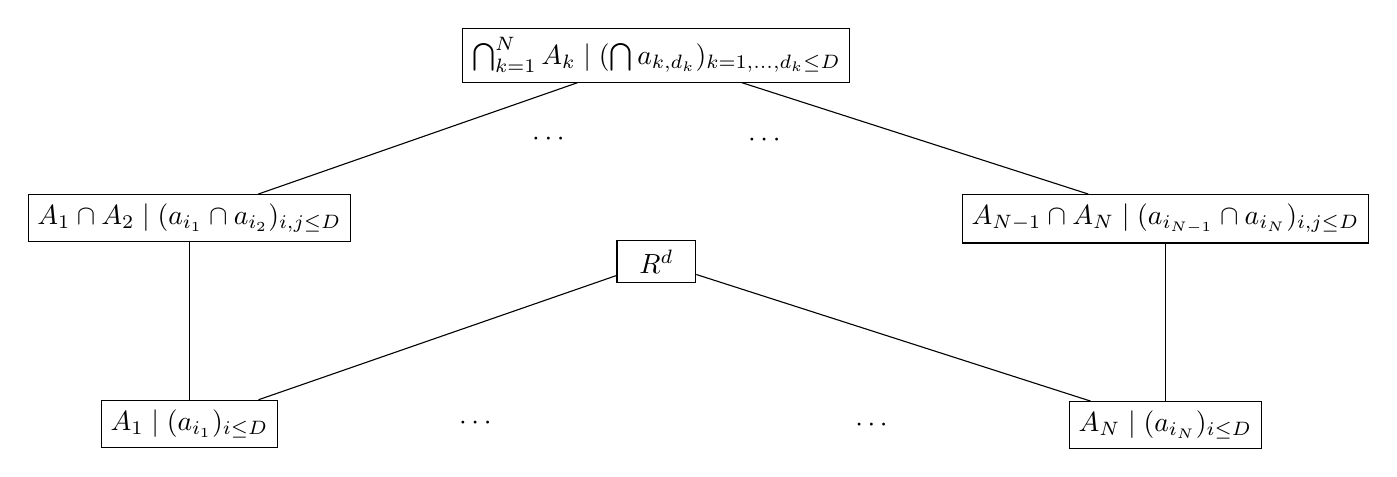
\begin{tikzpicture}[node distance=2cm, every node/.style={draw, minimum width=1cm, align=center}]
    % Nodes
    \node (top) {$\bigcap_{k=1}^N A_k \mid (\bigcap a_{k,d_k})_{k=1,\ldots,d_k \leq D}$};
    \node (left) [below left=of top] {$A_1 \cap A_2 \mid (a_{i_1} \cap a_{i_2})_{i,j \leq D}$};
    \node (right) [below right=of top] {$A_{N-1} \cap A_N \mid (a_{i_{N-1}} \cap a_{i_N})_{i,j \leq D}$};
    \node (bottomleft) [below=of left] {$A_1 \mid (a_{i_1})_{i \leq D}$};
    \node (bottomright) [below=of right] {$A_N \mid (a_{i_N})_{i \leq D}$};
    \node (bottom) [below=of top] {$\mathbb{R}^d$};

    % Dots for omitted parts
    \node (dots1) [right=of left, yshift=1cm, draw=none] {$\cdots$};
    \node (dots2) [left=of right, yshift=1cm, draw=none] {$\cdots$};
    \node (dots3) [right=of bottomleft, draw=none] {$\cdots$};
    \node (dots4) [left=of bottomright, draw=none] {$\cdots$};

    % Edges
    \draw (top) -- (left);
    \draw (top) -- (right);
    \draw (left) -- (bottomleft);
    \draw (right) -- (bottomright);
    \draw (bottomleft) -- (bottom);
    \draw (bottomright) -- (bottom);
\end{tikzpicture}
\end{document}